\documentclass{article}

\usepackage[%
    left=0.5in,%
    right=0.5in,%
    top=0.5in,%
    bottom=0.5in,%
]{geometry}%
\usepackage{minitoc}
\usepackage{multicol}
\usepackage{graphicx}
\usepackage{fixltx2e}
\usepackage{listings}
\usepackage{color}
\usepackage{hyperref}
    \hypersetup{ colorlinks = true, linkcolor = blue }
\usepackage{blindtext}
\definecolor{lightgray}{gray}{0.9}
\graphicspath{ {./} }

\newcommand{\inlinecode}[2]{\colorbox{lightgray}{\lstinline
[language=#1]$#2$}}
\newcommand{\worddef}[1]{\hyperref[sec:reference]{\textit{#1}}}

\definecolor{pblue}{rgb}{0.13,0.13,1}
\definecolor{pgreen}{rgb}{0,0.5,0}
\definecolor{pred}{rgb}{0.9,0,0}
\definecolor{pgrey}{rgb}{0.46,0.45,0.48}

\lstset{language=Java,
  showspaces=false,
  showtabs=false,
  breaklines=true,
  showstringspaces=false,
  breakatwhitespace=true,
  commentstyle=\color{pgreen},
  keywordstyle=\color{pblue},
  stringstyle=\color{pred},
  basicstyle=\ttfamily,
  moredelim=[il][\textcolor{pgrey}]{$ $},
  moredelim=[is][\textcolor{pgrey}]{\%\%}{\%\%}
}

\begin{document}

\tableofcontents

\newpage

\section{The Manifest file}

A	'list' declaring all public (visible) application’s	components. Uses:
\begin{itemize}
  \item Specify	entry	points: How	are	they started, what can access it (inside and outside the application)
  \item Information about the application: What is it allowed to do, what are its requirements (minimum, maximum SDK versions)
\end{itemize}
Manifest file should always be contained inside .apk (AndroidManifest.xml)

\section{Activities}

Have to be sub-classes of \texttt{android.app.Activity} and they present a visual UI.\\
Each activity has its own 'window'
\begin{itemize}
  \item Only one 'window' on screen at once
  \item Granular management of the resources of an application
  \item UI layout: a 'View' specified in a separate XML file and constructed programmatically
\end{itemize}
Apps can have several activities, typically, one activity in an app is specified as the \textbf{main activity}, which is the \textbf{first screen to appear} when the user launches the app. Each activity can then start another activity in order to perform different actions. \\
\textbf{For example}, the main activity in a simple e-mail app may provide the screen that shows an e-mail inbox. From there, the main activity might launch other activities that provide screens for tasks like writing e-mails and opening individual e-mails.

\begin{multicols}{2}

\subsection{Android UI}

Usually activities have a full screen window, which:
\begin{itemize}
  \item Can hover over another activity 
  \item Can be transparent
  \item Can be (Multi-window / picture-in-picture)
\end{itemize}
Within the window there is a hierarchy of View objects, which can be
\begin{itemize}
  \item Set with setContentView() 
  \item Inflated to fill the available window
\end{itemize}
Usually specified via an XML resource (/res/layout/mylayout.xml)

\subsection{View	Hierarchy}

Types	of	View	subclasses
\begin{itemize}
  \item Those	that	display	something	(Views)
  \item Those	that	do	something	(Widgets)
  \item Those	that	layout	subviews (ViewGroups)
\end{itemize}
\textbf{Shallow} layout hierarchies are	preferred: wide over deep with as few nested layouts as possible. We can	alter	the	view	hierarchy	programmatically as	the	application	runs:
\begin{itemize}
  \item addView, removeView
  \item find a particular view by ID generated from XML layout definition
\end{itemize}
We can also bind views to data
\end{multicols}

\section{Views}

\subsection{ViewGroups - Layouts}

\begin{itemize}
  \item \textbf{FrameLayout:} Simplest, contains a single object
  \item \textbf{LinearLayout:} Aligns all children in a single direction, based on the orientation attribute (Lists, left to right, top to bottom)
  \item \textbf{TableLayout:} Positions children into rows and columns
  \item \textbf{ConstraintLayout / RelativeLayout:} Lets the child views specify their position relative to the parent view or to each other. Has alignment constraints
  \item \textbf{ScrollView:} A vertically scrolling view, like FrameLayout only contains a single element (e.g. a LinearLayout)
  \item \textbf{SwipeRefreshLayout:} Detects the vertical swipe, displays a progress bar, and triggers callback methods.
  \item \textbf{AbsoluteLayout:} Positions and sizes child elements proportional to its own size and position or by absolute values.
\end{itemize}

\subsection{Views	- Widgets}

A child \textbf{View} that the user can (optionally) interact with
\begin{itemize}
  \item Button (a button) EditText (text entry)
  \item CalendarViewer (a calendar widget)
  \item ImageView (displays an image)
\end{itemize}
Handle	appropriate	UI	events
\begin{itemize}
  \item In code, register setOnClickListener()
  \item In XML layout, set android:onClick parameter
\end{itemize}
Properties / parameters, which are set via XML at build-time. Equivalent to using set get methods for modifying at run-time.

\subsection{Views - Parameters}

Parameters specify the details of particular Views
\begin{itemize}
  \item Width, height: generally not in terms of absolute pixels. For example:\\ 
  \texttt{android:layout\_width="match\_parent"}\\
  \texttt{android:layout\_height="wrap\_content"}
  \item Id: used to generate a Java member variable we can refer to programmatically. For example: \texttt{android:id="@+id/my\_button"}
  \item Methods: used to automatically bind UI events to code. For example: \texttt{android:onClick="myMethod"}
\end{itemize}

\section{Tasks, Activities and Processes}

\subsection{Overview}

Activity
\begin{itemize}
  \item An application component that defines a screen of information
  \item An app is a collection of activities, consisting of both the activities you create and those you re-use from other apps 
\end{itemize}
Task
\begin{itemize}
  \item The sequence of activities a user follows to accomplish a goal.
  \item A single task can make use of activities from just one app, or may draw on activities from a number of different apps
\end{itemize}
Process
\begin{itemize}
  \item Created to host components belonging to a particular app
  \item I.e. a task can span multiple processes
\end{itemize}

\subsection{Tasks vs Activities}

\begin{itemize}
  \item Activities can start other activities. Forms a stack of Activities, where current activity is on the top (The back stack)
  \item Task is an API that represents asynchronous method calls  
  \item Multiple activities form a Task as a task might span multiple applications.
  \item An activity should be an \worddef{atomic} part of a particular task. This supports reuse and integration into multiple tasks.
  \item Activities in a task move as a unit from foreground to background and vice versa. Switching	task = switching stack
\end{itemize}

\section{Activity	Lifecycle}
Essentially in one of three states: \textbf{Active, Paused, Stopped}. If paused or stopped, the system can drop the Activity from memory:
\begin{itemize}
  \item Stopped activities are suspended in memory. Consume no processing resources.
  \item Inactive activities are destroyed if memory is required. Least recently used
  \item This is important because android does not have SWAP
\end{itemize}
Transitioning	between	events	generates	events: setup ui, save state

\begin{center}
  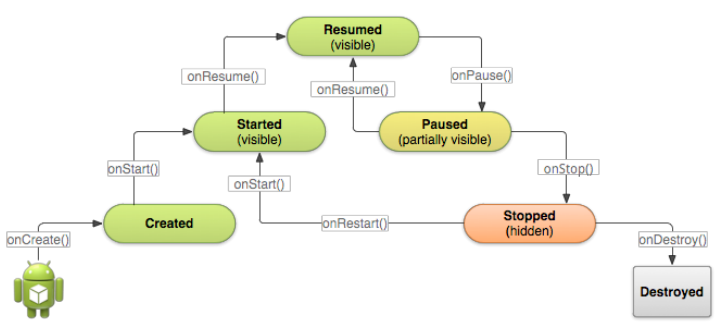
\includegraphics[scale=0.5]{activity_lifecycle.png}
\end{center}

\section{Hierarchical	Activity Navigation}

\begin{multicols}{2}
\begin{itemize}
\item \textbf{Descendant} navigation
\begin{itemize}
  \item Users descend down an activity hierarchy
  \item From parent to child activity
\end{itemize}
\item \textbf{Lateral} navigation
\begin{itemize}
  \item Collection-related siblings: Items in a collection
  \item Section-related siblings: Different sections of information about the parent
\end{itemize}
\item Forms	of	navigation
\begin{itemize}
  \item Lists selecting an activity
  \item Tab between screens
  \item Swiping between screens
  \item Buttons to start an activity
\end{itemize}
\end{itemize}

\vfill\null

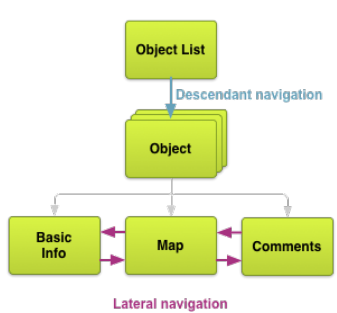
\includegraphics[scale=0.6]{navigation.png}

\end{multicols}

\subsection{Back and up}

Undo lateral and descendant navigation:
\begin{itemize}
  \item Back:
  \begin{itemize}
    \item Finishes the current activity
    \item Resumes the next activity on the stack
    \item NB tabs and swipes change information shown in the current screen, not the screen activity, so should not affect history
  \end{itemize}
  \item Up
  \begin{itemize}
    \item Finishes the current activity
    \item Starts (or resumes) the appropriate parent activity
    \item As specified in the manifest: If it’s in the back stack, bring it forward
    \item Can create a "fake" back stack
  \end{itemize}
\end{itemize}

\section{Intents}

Don’t initantiate the Activity sub-class. Android works by passing Intent objects around:
\begin{itemize}
  \item Intent is used to describe an operation: action and the data to operate on (as a URI)
  \item Allows for late runtime binding
  \item Glue multiple activities together
\end{itemize}
Android figures out how to honour the intent by inspecting registered manifests.
\begin{itemize}
  \item Starting an Activity
  \begin{itemize}
    \item Create a new Intent object
    \item Specify what you want to send it to. Either implicitly, or explicitly
    \item Pass the Intent object to startActivity() and new activity then started by the runtime 
  \end{itemize}
  \item Stopping an Activity
  \begin{itemize}
    \item The called Activity can return to the original one by destroying itself, by calling the method finish()
    \item Or when the user presses the back button
  \end{itemize}
\end{itemize}

\subsection{Intent types}

\begin{multicols}{2}

\subsubsection{Explicit}
Provide fully qualified classname of Activity to start
\begin{lstlisting}[language=Java, basicstyle=\small]
Intent myIntent =
  new Intent(context,otherActivity.class);
startActivity(myIntent);
\end{lstlisting}

\vfill\null
\columnbreak

\subsubsection{Implicit}
Data and action are used to resolve the most appropriate activity. Usually handled by the OS
\begin{lstlisting}[language=Java,basicstyle=\small]
Intent myIntent =
  new Intent(context,otherActivity.class);
startActivity(myIntent);
Uri webpage = Uri.parse("http://www.cs.nott.ac.uk");
Intent myIntent =
  new Intent(Intent.ACTION_VIEW, webpage);
Uri number = Uri.parse("tel:01151234567");
Intent myIntent =
  new Intent(Intent.ACTION_DIAL, number);
startActivity(myIntent);
\end{lstlisting}
\end{multicols}

\subsection{Intent Filters}

Manifest specifies intent filter:
\begin{itemize}
  \item Determine which Intents should be handled by the Activity class
  \item Match on action, schema of the URI
  \item When having multiple matches, user can choose the application.
\end{itemize}

\begin{lstlisting}[language=Java]
<activity android:name=".BrowserActivitiy"
          android:label="@string/app_name">
  <intent-filter>
     <action android:name="android.intent.action.VIEW" />
     <category android:name="android.intent.category.DEFAULT" />
     <data android:scheme="http"/>
  </intent-filter>
</activity>
\end{lstlisting}

\section{Inter-Activity	Communication}

\begin{itemize}
  \item \texttt{startActivity()} doesn’t allow the Activity to return a result
  \begin{itemize}
    \item Applications usually want to maintain state
    \item Remember what the user has done across all activities
    \item We could store state in the broader Application context
    \item But activities may be communicating between processes (IPC)
    \item Entry point for other applications
  \end{itemize}
  \item \texttt{startActivityForResult()}
  \begin{itemize}
    \item Still takes an Intent object, but also a numerical request code
  \end{itemize}
  \item \texttt{onActivityResult()} then called on the calling activity.
  \begin{itemize}
    \item Data can be packaged up in an Intent / Bundle
    \begin{itemize}
      \item Activity creates an Intent object containing the result
      \item Use a Bundle to “bundle” complicated objects
    \end{itemize}
     \item Intent object then passed to \texttt{onActivityResult()} on finish
     \begin{itemize}
       \item Returns an integer result code, set with \texttt{setResult()}
       \item Returns the request code so we know which Activity we are receiving a result from
     \end{itemize}
  \end{itemize}
\end{itemize}

\section{Saving UI state}
Shouldn’t rely on an Activity storing UI state
\begin{itemize}
  \item E.g. rotating the device will destroy and recreate activity
  \item Aggressive OS management: application context handles various onTrimMemory calls
\end{itemize}
Before \texttt{onStop()} is called, Android will call \texttt{onSaveInstanceState()}
\begin{itemize}
  \item To restore the UI to its previous state on restore. This is a cascading	call into UI components
\end{itemize}
This allows you to save any UI state into a Bundle object
\begin{itemize}
  \item It's essentially a key/value store, where key is string id of the element and value is any serializable data
  \item When the Activity is recreated, the Bundle is passed to \texttt{onCreate()} and \texttt{onRestoreInstanceState()}, giving the activity a chance to restore its state
\end{itemize}
Save other state to more \textbf{persistent storage}: SQLite / user preferences.


\newpage

\section*{Reference section} \label{sec:reference}
\begin{description}
	\item[atomic] \hfill \\ Something that "appears to the rest of the system to occur instantaneously" (One operation at a time).\textbf{Atomic operation} means an operation that appears to be instantaneous from the perspective of all other threads. You don't need to worry about a partly complete operation when the guarantee applies.
\end{description}
\end{document}
